\documentclass[a4paper, parskip=true, firsthead=false, fromemail=true, foldmarks=false]{scrlttr2}
\usepackage[utf8]{inputenc}
\setkomavar{fromemail}{thomas.gibaud@ens-lyon.fr}
\setkomavar{signature}{Mathieu Leocmach,\\ Mathieu Nespoulous,\\ Sébastien Manneville,\\ Thomas Gibaud\\
{\small Ecole Normale Supérieure de Lyon}}


\usepackage{amsmath}
\usepackage{amsfonts}
\usepackage{amssymb}
\usepackage{graphicx}
\usepackage[british]{babel}

\usepackage{kpfonts}
\usepackage{tabu}
\usepackage{wrapfig}

\begin{document}
\begin{letter}{From:\\
Thomas Gibaud,\\
Laboratoire de physique,\\
Ecole Normale Supérieure de Lyon/CNRS, France\\
\texttt{thomas.gibaud@ens-lyon.fr}
}
\opening{\bf Dear Editor,}

Please find enclosed our manuscript, entitled \emph{Hierarchical wrinkling in a confined permeable biogel}, which we are submitting for publication as an article to Nature Materials.



Supplementary Video 1 arouses one's curiosity. It shows microscopy images of a thin optical cell containing a protein gel whose adhesion to the lateral wall is prohibited. No external stimulus is applied. How can a simple biogel spontaneously form such complicated nested patterns?


\begin{tabu}{@{}X[m]m{0.2\textwidth}}
%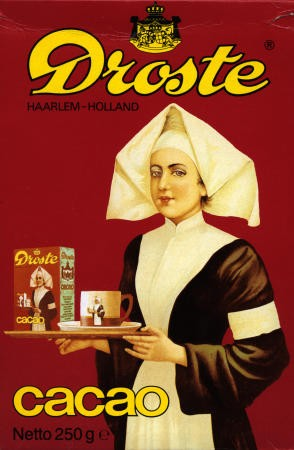
\includegraphics[height=8.5\baselineskip]{../Droste.jpg} &
Supplementary Video 2, which shows a 3D construction of the gel based on confocal imaging, hints towards the answer. The gel shrinks then swells and wrinkles due to the excess area created during swelling. This is however not the end of the story as boundary conditions frustrate the development of the wrinkles and induce buckling within the buckling. This hierarchical pattern is a beautiful and natural illustration of the well known Droste effect, known in France as ``Vache qui rit'' effect, where an image contains a smaller version of itself.&
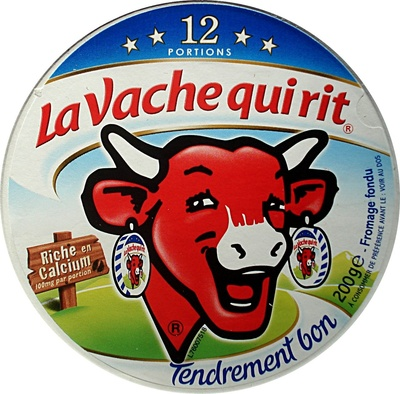
\includegraphics[width=0.2\textwidth]{../vachequirit.jpg}
\end{tabu}


%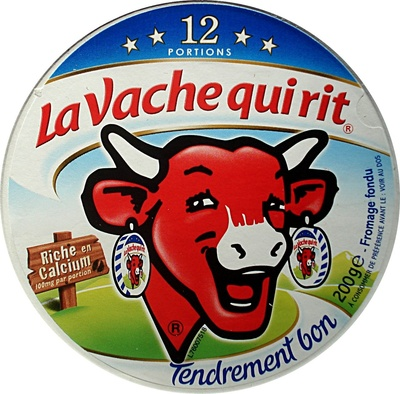
\includegraphics[width=0.2\textwidth]{../vachequirit.jpg}


%\begin{tabu}{X[c]X[c]}
%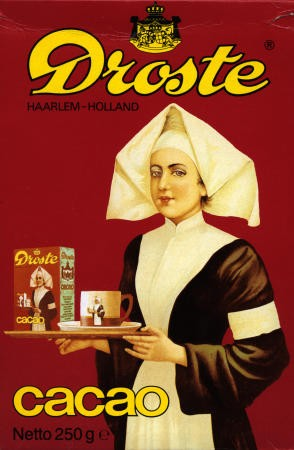
\includegraphics[height=8\baselineskip]{../Droste.jpg}&
%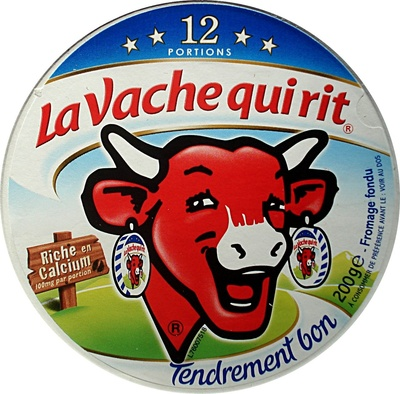
\includegraphics[height=8\baselineskip]{../vachequirit.jpg}
%\end{tabu}



It is universally recognized that confined thin surfaces may wrinkle due the growth of an excess of material. For example on the biology side a difference in growth rates between the gut tube and its dorsal anchoring is responsible for the vilification of guts. Localized cell death in biofilms focuses mechanical forces and initiates 3D labyrinth pattern. Such patterns can also be triggered by physical parameters such as temperature dilation, swelling or the removal of pre-strain.

So far, laboratory experiments on synthetic systems have focused on free interfaces where gravity dominates over viscosity as the wavelength selection mechanism. However, in biologically relevant situations for instance, gravity can generally be neglected and cannot be invoked as the driving mechanism for wrinkling. Therefore, benchmark experiments, such as the ones presented in Supplementary Videos 1 and 2, that explore the possibility of wrinkling in confined porous soft materials immersed in a buoyancy-matched viscous medium are in line.

From a fundamental perspective, our work unifies concepts from diverse soft matter systems.
\begin{enumerate}
\item From food science we have hijacked the process of yoghurt making to form gels. Usually, when one acidifies milk, the caseins flocculate. To form a uniform yoghurt gel one needs to lower homogeneously the pH, as bacteria do. Here we use the acidulent GDL for finer control.

\item  Next, we exploit the concept of stability in colloidal suspensions. As the GDL acidifies the medium, caseins loose their net charge and aggregate. Upon further acidification the caseins regain charges and partially desorb from the gel. This makes the gel successively shrink and swell.

\item This process also can be well understood by invoking two different theories of gelation. Diffusion limited cluster aggregation is responsible for the formation of the fractal network of the gel ; whereas arrested phase separation well describes the coexistence between a dilute phase and a dense glassy network.

\item Finally, we invoke hydrodynamics with the seminal work of Darcy and Poiseuille. In particular we demonstrate the kinetic selection of the wavelength due to two sources of viscous dissipation. We predict the wrinkling wavelength invoking Poiseuille flows of the solvent above and below the gel layer for long wavelengths and a new mechanism, Darcy flows of the solvent through the gel layer for short wavelengths.
\end{enumerate}



From a practical perspective, such a model experiment, because it relies on pH induced charge stabilisation/destabilisation, should be generalisable to different kind of proteins. Controlled gelation with peculiar boundary conditions introduces a robust method to produce wrinkled surfaces that is distinct from other emerging technologies. We use a combination of complementary techniques ranging from polymer brush grafting, titration, light microscopy, rheology, permeability measurements and confocal microscopy that allow us to fully understand the relations between all levels of hierarchy from the individual proteins to the macroscopic level. Indeed, we directly measure and relate the non-monotonic pH response of the proteins to the spontaneous shrinkage and swelling effect of the casein network at the micron level to the wrinkles at the millimetre scale. Playing with the geometry, the gel composition and the viscosity of the solvent, we explore a wide range of physical parameters to check the validity of our models and evidence the first example of wrinkling driven by Darcy flow.


The impact of our work extends beyond soft-matter physics. For instance, it illustrates daily life problems such as wrinkles encountered while putting up wall paper: water swells the paper and air infiltrates through the paper and produces Darcy blisters. Our results could also set a reference for potential applications. For example since the wrinkling pattern is unique and unreproducible it could be used as a safe key for identification. Moreover, the nested nature of the patterns could be used in optical devices such as diffraction gratings or Fresnel lenses. Finally, our experiments pave the way for exploring the possibility of wrinkling in confined porous soft materials immersed in a buoyancy-matched viscous medium such as biological tissues. Indeed during morphogenesis of the embryo the development of confined permeable and wrinkled surface is ubiquitous.


For all these reasons we believe that our manuscript is suitable for a publication in an interdisciplinary journal such as Nature Materials. With this manuscript we are including 7 Supplementary Videos, which have been mailed to your editorial office. As potential reviewers we wish to suggest: L. Mahadevan (Harvard, USA), N. Menon (Amherst, USA), Benoît Roman (ESPCI, France), Enrique Cerda (Univ. Santiago-Chile, Chile), Mokhtar-Adda-Bedia (ENS Paris, France), Dominic Vella (Oxford, UK), Eric Lauga (Cambridge, UK).

 

We thank you for your consideration, time and attention.

\closing{\bf Sincerely yours,} 

\end{letter} 
\end{document}